\documentclass[main.tex]{subfiles} 
\begin{document}

\section*{Metode \& Gjennomføring}
\label{sec:2}

Nordahl skriver at utfordringen er ikke at skolen mangler data, men at data ofte i lite grad blir
systematisk analysert og senere aktivt brukt for å forbedre praksisen (\citeNP[s. 9]{hell07}).
I denne oppgaven er dataen innsamling av elevbesvarelser og mine egne skriftlige tilbakemeldinger.
Jeg har valgt å fremheve noen av disse skriftlige tilbakemeldinger for å analysere min egen praksis.
Dataen er også ment til å brukes i læringsrettet kontekst, der elevene kan få
individuelle tilbakemeldinger og fremovermeldinger. 
\newline
\newline
I denne oppgaven har jeg valgt å også benytte meg av kvalitativ forskning og metode. Ved
kvalitative metoder får en ofte anledning til å gå mere i dybden på materialet og man kommer
tett på subjektene, men derfor er metoden også mere ressurskrevende og man må derfor
begrense antall forsøksobjekter. Forskerne kaller det å "mette" materialet, noe som vil si 
flere intervjuer neppe vil avdekke noe avgjørende nytt (\citeNP{hoff13}). Jeg har hatt
personlige samtaler med 10 av 27 elever som tok kartleggingstesten. Elevene hadde ulike
resultater og derfor også ulike former for tilbakemeldinger og fremovermeldinger.
\newline
\newline
Jeg valgte å fokusere på elevenes kunnskap rundt følgende kompetansemål (utdanningsdirektoratet, 2013) :
\begin{itemize}
\item finne og diskutere sannsyn gjennom eksperimentering, simulering og berekning i daglegdagse samanhengar og spel
\item beskrive utfallsrom og uttrykkje sannsyn som brøk, prosent og desimaltal
\end{itemize}
Ved design av testen i sannsynlighet, ble disse kompetansemålene brukt som veiledning til
utformingen av kartleggingsprøven.
\newline
\newline
Når elever skal vurderes så kan dette gjøres på flere måter:
\begin{itemize}
\item Normalfordeling og fast poengsum : da blir vurderingsgrunnlaget \emph{de andre elevenes prestasjoner}. 
Dette blir også referert som relativ vurdering. Vurdering av en individ avhenger da av de andre
elevenes prestasjoner. Ved fast poengsum innebærer det at det er etter poeng oppnåelse elevene blir vurdert. 
Da vil karakterene avgjøres ut ifra hvor mye peongsum eleven har klart å oppnå. Her vil ofte vanskelig oppgaver
bli vektlagt mer enn enkelere oppgaver.
\item Individrelatert kriterier : da vurderes eleven utelukkende i forhold til sine egne forutsetninger
og tidligere prestasjoner. I grunnskolen skal vurderingen uten karakterer i hovedsak være 
individrelatert  (\citeNP[s. 25]{hell07}).
\item Målrelatert kriterier : kvalitetsstandarden blir da en didaktisk kontretisering av kompetansemål.
 I grunnskolen skal vurderingen med karakterer skje etter målrelaterte kriterier (\citeNP[s. 26]{hell07}).
\item Kompetansemål : da vurderes elevene utfra hvilket nivå eller trinn (i henhold til Bloom's taksonomi) 
                      de demonstrer i sin oppnåelse av kompetansemålene.
\end{itemize}
Jeg er nok enig i at bruken av individrelatert vurdering er en god vurderingsgrunnlag i situasjoner
der karakterer ikke brukes. Denne vurderingsformen oppfyller kriterier for god vurdering,
siden den brukes til å fortelle eleven hvor hen befinner seg i sitt studieløp/progresjon.
Når lærer og elev sammen setter individuelle mål, både nærliggende og langsikte, da vil eleven
gjennom et slikt vurderingsgrunnlag få konkete tilbakemeldinger og fremovermeldinger som 
fokuserer på nettopp elevens prestasjoner og målsettinger som hen har laget sammen med
læreren. Det kan også være fordelsaktig å koble målsettingene til kompetansenivå eleven demonstrerer
og jobbe mot høyre kompetansenivå. For eksempel diskutere er et høyt kompetansenivå, der eleven 
kan trekke sammnenhenger og redegjøre for sine tanker om en problemstilling. I motsetning er
å beskrive et middels kompetansenivå (i Bloom's taksonomi).
\newline
\newline
Siden min hensikt var å kartlegge elevenes svakheter, da er det passende å isteden bruke individrelaterte kritier 
og koble inn kompetansemålene. Til en kartleggingsprøve så er det vanskelig å trekke inn individrelaterte kriterier
med mindre lærer har godt kjennskap til eleven på forhånd. Jeg koblet dessverre ikke inn kompetansemålene heller, 
noe som det bør brukes mer av. Gjennom noen av mine samtaler med elever, oppdaget jeg fort at det var få som trakk 
forbindelsen mellom egen læring og koblingen til kompetansemålene. For undervisere regnes det som en god praksis at 
elevene er alltid bevisste om hvorfor de lærer det de lærer og hvor de er på vei. \citeA[s. 136]{klet13} beskriver 
en god undervisningsseksens der lærere klarer å balansere mellom tilegnelses-, utprøvings-, og 
konsolideringssituasjoner. Ifølge Klette har norske klasserom ensidige tendenser i bruken av varierte arbeidsmåter. 
Slik det kan ses fra figur \ref{fig:odeg10}, er det for eksempel lite konsolideringssituasjoner. Lærernes 
metalæringsaktiviteter regnes som særlig avgjørende for å sikre elevenes læring (\citeNP[s. 186]{klet13}). Å bruke 
dette som et fast organiserende prinsipp, blir derimot sjelden gjennomført (\citeNP[s. 26]{odeg10}).
\begin{figure}[h!]
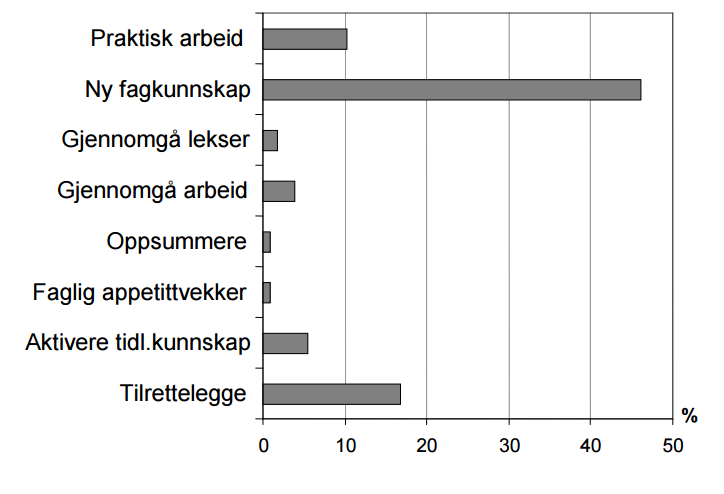
\includegraphics[scale = 0.6]{../figures/undervisnings_aktivitet.png}
\caption{Oversikt over naturfaglærernes undervisningstilbud til elevene fra PISA+ studie. Kilde: 
\protect\citeA{odeg10}.}
\label{fig:odeg10}
\end{figure}

\subsection*{Kartleggingsprøven i sannsynlighetsregning}

Ifølge \citeA[s. 15]{brek02} kan diagnostiske oppgaver bli brukt til å identifisere og fremheve misoppfatninger 
som elevene har utviklet, gi læreren informasjon om elevenes løsningsstrategier og måle hvordan undervisningen 
har hjulpet elevene til å overvinne misoppfatningene. Gjennom blant annet kartleggingsprøver får elever muligheter
til å utrykke sine skriftlige ferdigheter i matematikk. Å skrive matematikk regnes som en av grunnleggende 
ferdighetene. Det innebærer blant å beskrive og forklare egen tankgegang, å lage tegninger og skissere grafer. 
Skriving i matematikk blir sett på som et redskap for å utvikle egne tanker og egen læring (\citeNP{udirGF}). 

Før kartleggingsprøven ble brukt, jobbet elevene en uke med sannsynlighetsregning. Mine observasjoner fra denne uken, 
og basert på kompetansemål, formet jeg testen sammen med en annen praksisstudent. Henikten med kartleggingsprøven 
var å få oversikt over elevers ferdigheter i sannsynlighetsregning og hjelpe de med å avdekke deres
svakheter og misoppfattelser. Kartleggingsprøver kan brukes i mange forskjellige situasjoner. 
Pyskologene Daniel Kahneman og Amos Tversky har satt fram en teoretisk ramme for å undersøke 
læring av sannsynlighet og statistikk. Deres tese er at mennesker uten erfaring, refleksjon og innsikt i statistikk,
bruker følgende strategier for å bedømme sannsynlighet (\citeNP{udir13}; \citeNP{evan17}):
\begin{itemize}
\item Representativitet : små utvalg skal representere den fordelingen som finnes i populasjonen
\item Tilgjengelighet : sannsynlighet bedømmes ut fra hvor lett det er å huske spesielle tilfeller
\item Resultatorientering : utfallet kan forutses, som ved en deterministisk prosess
\item Konjunksjonsfellen : sannsynligheten for at to hendelser inntreffer samtidig er mindre enn sannsynligheten
for at en av hendelsene inntreffer.
\item Vanskeligheter med betinget sannsynlighet
\end{itemize}
Dette er ofte misoppfattelser som også ligger hos elever med ulike faglig bakgrunn.
I tabellen fra figur \ref{fig:skov98}, kartlegger \citeA{skov98} type oppgaver etter det han kaller 
\mbox{\emph{opgaveparadigmet} :}
klassiske åpne og lukkede oppgaver vs. \emph{undersøgelseslandskaber} eller utforskende oppgaver. I tabellen tallfester
han disse oppgavetypene etter i hvilken grad de er tilnærmet virkeligheten. Jeg kommer til å bruke tabellen når jeg
drøfter oppgavene fra kartleggingsprøven (se Vedlegg 1). \citeA{skov98} beskriver oppgaveparadigmet som
en læringsmiljø der læreren innleder med å gjennomgå nytt stoff, deretter gjennomgås utvalgte oppgaver, hvor elever 
regner oppgaver, enten individuelt eller i grupper. \emph{En matematikkundervisning, der er strukturert efter 
opgaveparadigme, føjer seg ind i \guillemotleft oppgavediskursen\guillemotright} (\citeNP[s. 28]{skov98}).
\begin{figure}[h!]
\centering
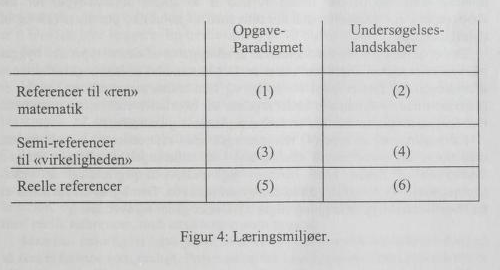
\includegraphics[scale = 0.9]{../figures/laeringsmiljoer.png}
\caption{Kilde: \protect\citeA{skov98}.}
\label{fig:skov98}
\end{figure}

\end{document}
